% SoundCode workflow figure -- THE figure of the paper.
% Asynchronous verifier in a background task. LLM keeps streaming.
% A ghost red arrow shows where ROCODE would block; SoundCode's
% real path is async (teal) and rollback (blue).
\documentclass[border=2pt]{standalone}
\usepackage{tikz}
\usepackage{xcolor}
\usepackage{amssymb}
\usetikzlibrary{shapes.geometric, arrows.meta, positioning, fit, backgrounds, calc}

\begin{document}
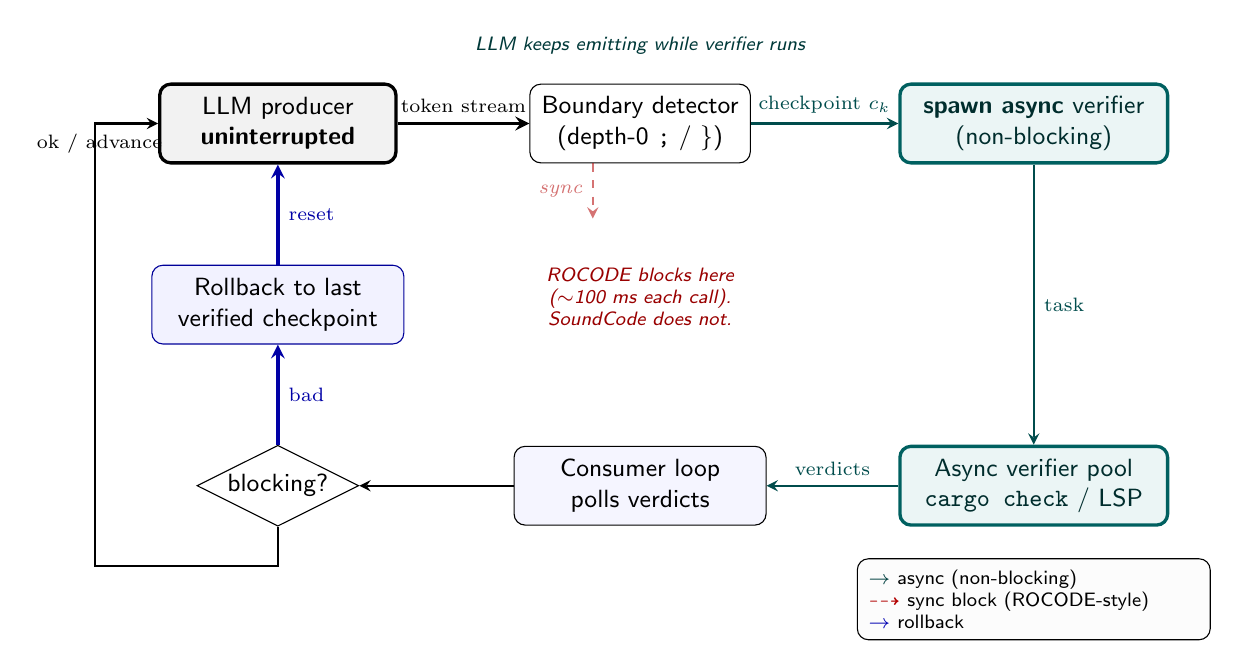
\begin{tikzpicture}[
    >=stealth,
    font=\sffamily\small,
    box/.style       ={draw, rounded corners, align=center, minimum height=10mm,
                       minimum width=28mm, inner sep=3pt, fill=white},
    llmbox/.style    ={box, fill=black!5, minimum width=30mm, very thick},
    asyncbox/.style  ={box, draw=teal!75!black, very thick, fill=teal!8,
                       minimum width=34mm, text=teal!35!black},
    ckptbox/.style   ={box, fill=blue!5, draw=blue!60!black, minimum width=32mm},
    decision/.style  ={diamond, draw, aspect=2.0, inner sep=1pt, align=center,
                       fill=white, minimum height=10mm},
    flow/.style      ={->, thick},
    asyncflow/.style ={->, thick, teal!60!black},
    ghost/.style     ={->, thick, red!70!black, dashed, opacity=0.55},
    rollflow/.style  ={->, very thick, blue!65!black},
    note/.style      ={font=\sffamily\scriptsize\itshape, text=teal!45!black},
    redannot/.style  ={font=\sffamily\scriptsize\itshape, text=red!60!black},
    legendbox/.style ={draw, rounded corners, fill=black!1,
                       inner sep=4pt, font=\scriptsize\sffamily,
                       align=left}
]

% =================== TOP ROW: hot path (producer) ===================
\node[llmbox]   (llm)   at (1.0,0)   {LLM producer\\\textbf{uninterrupted}};
\node[box]      (bnd)   at (5.6,0)   {Boundary detector\\(depth-0 \texttt{;} / \texttt{\}})};
\node[asyncbox] (spawn) at (10.6,0)  {\textbf{spawn async} verifier\\(non-blocking)};

% Token-stream + checkpoint arrows
\draw[flow, very thick] (llm.east) -- (bnd.west)
    node[midway, above, font=\scriptsize] {token stream};
\draw[asyncflow] (bnd.east) -- (spawn.west)
    node[midway, above, font=\scriptsize] {checkpoint $c_k$};

% Annotation above producer (the headline message)
\node[note, above=2.5mm of bnd, text width=50mm, align=center]
    {LLM keeps emitting while verifier runs};

% Ghost red arrow: where ROCODE would block (small downward arrow from bnd)
\node[redannot, below=12mm of bnd, text width=46mm, align=center] (ghostnote)
    {ROCODE blocks here ($\sim$100 ms each call).\\SoundCode does not.};
\draw[ghost] ($(bnd.south)+(-6mm,0)$) -- ++(0,-7mm)
    node[pos=0.5, left, font=\scriptsize\itshape] {sync};

% =================== BOTTOM ROW: verifier + consumer + rollback ===================
\node[asyncbox] (pool) at (10.6,-4.6) {Async verifier pool\\\texttt{cargo check} / LSP};
\node[box, fill=blue!4, minimum width=32mm] (poll) at (5.6,-4.6)
    {Consumer loop\\polls verdicts};
\node[decision] (gate) at (1.0,-4.6) {blocking?};

% Rollback box on far left at producer level
\node[ckptbox] (rb) at (1.0,-2.3) {Rollback to last\\verified checkpoint};

% --- Arrows ---

% Spawn -> pool (down)
\draw[asyncflow] (spawn.south) -- (pool.north)
    node[midway, right, font=\scriptsize] {task};

% Pool -> consumer (verdicts)
\draw[asyncflow] (pool.west) -- (poll.east)
    node[midway, above, font=\scriptsize] {verdicts};

% Consumer -> gate
\draw[flow] (poll.west) -- (gate.east);

% Gate -> rollback (bad branch up)
\draw[rollflow] (gate.north) -- (rb.south)
    node[midway, right, font=\scriptsize] {bad};

% Rollback -> LLM
\draw[rollflow] (rb.north) -- (llm.south)
    node[midway, right, font=\scriptsize] {reset};

% OK branch: gate -> down/around -> back to LLM
\draw[flow] (gate.south) -- ++(0,-5mm) -| ($(llm.west)+(-8mm,0)$) -- (llm.west)
    node[pos=0.07, below, font=\scriptsize] {ok / advance};

% Legend below the right side
\node[legendbox, below=4mm of pool, text width=42mm, anchor=north] (legend)
    {\textcolor{teal!50!black}{$\rightarrow$} async (non-blocking)\\
     \textcolor{red!70!black}{$\dashrightarrow$} sync block (ROCODE-style)\\
     \textcolor{blue!70!black}{$\rightarrow$} rollback};

\end{tikzpicture}
\end{document}
